\documentclass[11pt,a4paper]{article} 
\usepackage{amsmath, amsthm, amssymb, calrsfs, wasysym, verbatim, bbm, color, graphics, geometry, physics, braket, titling, parskip,subfig}

\usepackage{hyperref}
\usepackage[T1]{fontenc}
\usepackage{mwe}
\usepackage{float}

\numberwithin{equation}{section} 

\usepackage{titlesec}
\titlelabel{\thetitle.\quad}     %to add dot to the section titles

\makeatletter
\renewcommand*\env@matrix[1][*\c@MaxMatrixCols c]{%
  \hskip -\arraycolsep
  \let\@ifnextchar\new@ifnextchar
  \array{#1}}
\makeatother

\definecolor{bluetext}{RGB}{30, 120, 150}

\geometry{tmargin=1.15in, bmargin=1.15in, lmargin=1.15in, rmargin = 1.15in}          %setting for the indentation 

\newcommand{\R}{\mathbb{R}}

\newcommand{\Z}{\mathbb{Z}}
\newcommand{\N}{\mathbb{N}}
\newcommand{\Q}{\mathbb{Q}}
\newcommand{\Cdot}{\boldsymbol{\cdot}}
\newcommand{\subtit}[1]{\textbf{\noindent{\large #1}}}
\newcommand{\subsubtit}[1]{\textbf{\noindent{ #1}}}

\DeclareMathAlphabet{\pazocal}{OMS}{zplm}{m}{n}
\newcommand{\La}{\mathcal{L}}
\newcommand{\Lb}{\pazocal{L}}


\newtheorem{thm}{Theorem}
\newtheorem{defn}{Definition}
\newtheorem{conv}{Convention}         %useful notation when writing         proofs, thms etc.
\newtheorem{rem}{Remark}
\newtheorem{lem}{Lemma}
\newtheorem{cor}{Corollary}
\newtheorem{pf}{Proof}


\title{MAT 309: PA 1}
\author{Mert Kurttutan}
\date{\vspace{-5ex}}


\begin{document}
\maketitle
\subtit{Question A}

\subtit{a)} The first part includes a 1D system where the heat is transported by conduction in steady state. By the Fourier's Law, we have

\begin{equation}
-k \dv{T}{x} = q_0
\end{equation}

Since the area is constant, for infinitesimal piece in 1D rod, we have

\begin{equation}
Q_{\text{in}} = Q_{\text{out}} \to q_{\text{in}} = q_{\text{out}} \to \dv{T}{x} = \text{constant} = \frac{T_R-T_L}{L}
\end{equation}

Finally, discretizing our system and using Taylor Expansion which terminates in the first derivative since the derivative of temperature is constant, we obtain
\begin{equation}
T_i = \dv{T}{x}\Delta x + T_{i-1}
\end{equation}

where $T_i$ is the temperature at i-th node, and $\Delta x$ is the interval between closest nodes. This is implemented inside the for loop.

\subtit{b)}The only change in the second part is the left-boundary condition. Imposing convection boundary condition and equating the heat fluxes at the left boundary, it follows
\begin{equation}
q_{\text{in}} = q_{\text{out}} \to k\dv{T}{x} = h(T_L-T_{\infty})
\end{equation}
Since the heat transport is still by conduction and given by Fourier's Law, it follows
\begin{equation}
k\frac{T_R-T_L}{L} = h(T_L-T_{\infty}) \to T_L = \frac{\frac{k}{L}T_R  + h T_{\infty}}{\frac{k}{L} + h } = 431.25\, \text{K}
\end{equation}
Having determined the boundary temperatures, we can discretize and calculate the temperature at nodes
\begin{equation}
T_i = \dv{T}{x}\Delta x + T_{i-1}
\end{equation}
where $\dv{T}{x} = \frac{T_R-T_L}{L}$ as before. 

The result of these are shown in the plot below.
\begin{center}
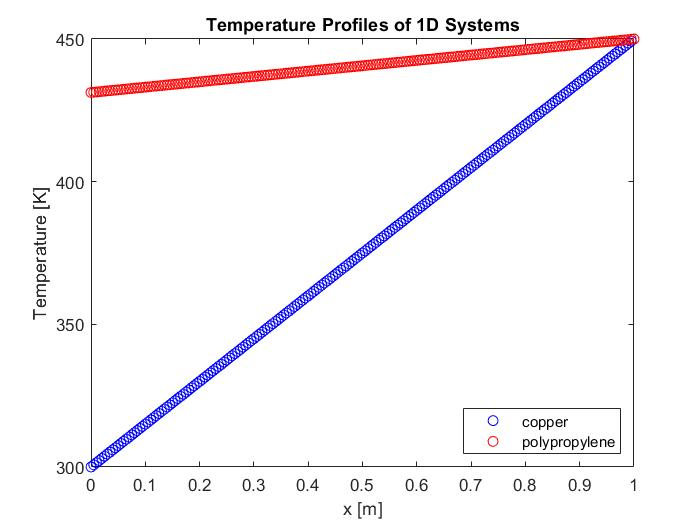
\includegraphics[scale=0.3]{plot.jpg}   
\end{center}

As you can see, the temperature profile is linear. The reason is that the only transport mechanism is by conduction, and the area is constant. Additionally, the type of boundary condition on the left creates leads to different temperatures on the left while the temperature gradient is constant within the material in steady state.

\end{document}
